% Document class and two-column conversion
\documentclass{report}
% dimensions of paper and relative text positioning
\usepackage[a4paper,top=2cm,bottom=2cm,left=2cm,right=2cm]{geometry}
% math symbols
\usepackage{amsmath}
\usepackage{amssymb}
% package for including URLs
\usepackage{url}
% Required for including images
\usepackage{graphicx}
\usepackage{float} % Required for specifying the exact location of a figure

% enable writing in greek
\usepackage[greek,english]{babel}
\usepackage[utf8]{inputenc}

\setlength{\parindent}{0pt} % Removes all indentation from paragraphs

% Start of the document
\begin{document}

% Set the language to greek
\selectlanguage{greek}

% Title page
\title{\Huge \bfseries \selectlanguage{english} Hardware 1 \\ Project 2024\selectlanguage{greek}} %\Huge and \bfseries are used to make the title bigger and bold
\author{Παπαδάκης Κωνσταντίνος Φώτιος\vspace{0.5cm} \\  ΑΕΜ:10371} % \vspace{0.5cm} is used to add some vertical space between the author and the AEM
\date{\today}
% prints the title, author and date on a separate page
\maketitle

\section*{Άσκηση 1}
Στην πρώτη άσκηση μας ζητείται να παράξουμε μια αριθμητική λογική μονάδα. 
Δημιουργούμε ένα $module$ το οποίο έχει 3 εισόδους και 2 εξόδους, 9 σταθερές
που δηλώνουν στον πολυπλέκτη ποια πράξη θα γίνει στην $alu$ και μια $switch$ 
η οποία ανάλογα με την τιμή που δέχεται ο πολυπλέκτης επιλέγει την αντίστοιχη
πράξη, όπως προδιαγράφεται στην εκφώνηση.
\\
Επιπρόσθετα φτιάχνουμε και ένα $testbench$ το οποίο ελέγχει όλες τις πιθανές
περιπτώσεις των εισόδων που μπορεί να δεχθεί το συγκεκριμένο module. Με $port
mapping$ περνάμε τις παραμέτρους της $alu$ στο $testbench$, φτιάχνουμε μια
συνάρτηση που να ελέγχει αν ταυτίζεται το αναμενόμενο αποτέλεσμα με το πραγματικό
και παράλληλα κρατάμε στο νου η παράμετρος $zero$ να είναι $1$ όταν το αποτέλεσμα
είναι $0$.

\section*{Άσκηση 2}
Για τη δεύτερη άσκηση συνθέτουμε μια αριθμομηχανή η οποία αξιοποιεί την $alu$ της
προηγούμενης άσκησης. Δημιουργούμε δύο αρχεία:
\begin{itemize}
    \item \selectlanguage{english}\textbf{calc\_enc:}\selectlanguage{greek} Υλοποιεί με $structural$ $verilog$ το σήμα $alu_op$ βάσει 
    της κατάστασης των τριών κουμπιών ($btnr$, $btnc$, $btnl$), 
    \item \selectlanguage{english}\textbf{calc:}\selectlanguage{greek} Συγκεντρώνει τη λειτουργικότητα των $alu$, $calc_enc$ και 
    επιπρόσθετα ενημερώνει τον συσσωρευτή βάσει της κατάστασης των κουμπιών $btnu$ και $btnd$.
    Επίσης φροντίζει να αντικατοπτρίζεται ο συσσωρευτής στο $LED$ και δημιουργεί με επέκταση 
    προσήμου δύο $32-bit$ εκδοχές του συσσωρευτή και του διακόπτη για να τις προωθήσει στην
    $alu$ η οποία δέχεται $32-bit$ εισόδους.
\end{itemize}

Κυματομορφές προσομοίωσης:
\begin{figure}[H]
    \centering
    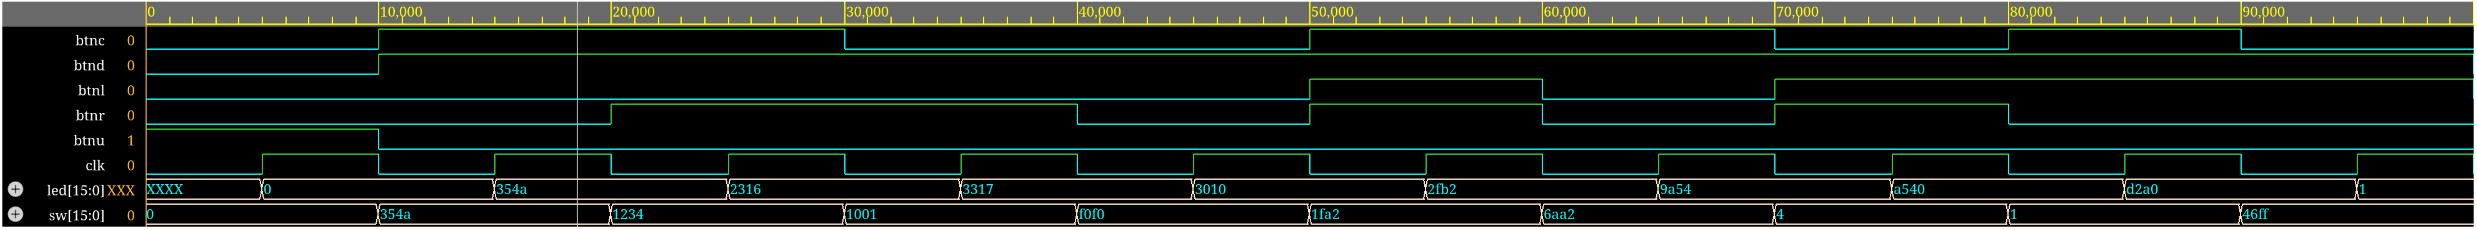
\includegraphics[width=1\textwidth]{media/exercise2_waveforms.png}
\end{figure}

\section*{Άσκηση 3}
Στη τρίτη άσκηση υλοποιούμε ένα αρχείο καταχωρητών το οποίο θα αποθηκεύει τις 
τιμές των καταχωρητών του επεξεργαστή $RISK\_V$ πάνω στον οποίο βασίζεται η
εργασία μας. Ο κώδικας είναι αρκετά απλός:
\begin{itemize}
    \item Αρχικοποιούμε τους καταχωρητές με την τιμή 0.
    \item Κάθε φορά που υπάρχει αλλαγή σε κάποια είσοδο του $module$ μας,
    διαβάζουμε τις τιμές που προσδιορίζουν οι $readReg1$ και $readReg2$. 
    Δίνουμε προτεραιότητα στην εγγραφή διαβάζοντας απευθείας από το
    $writeData$ στην περίπτωση που το $write enable$ παίρνει τιμή $1$.
    \item Στην θετική ακμή του ρολογιού, όταν το $write enable$ είναι $1$
    και το $writeReg$ δεν είναι $0$, τότε γράφουμε την τιμή του $writeData$
    στον καταχωρητή που προσδιορίζει το $writeReg$.
\end{itemize}
Για να είμαστε σίγουροι ότι ο κώδικάς μας είναι ορθός φτιάχνουμε ένα $testbench$
το οποίο ελέγχει 5 πράγματα:
\begin{itemize}
    \item Ότι όλοι οι καταχωρητές είναι αρχικοποιημένοι στο 0.
    \item Ότι μπορώ να γράψω μια τιμή σε έναν καταχωρητή και έπειτα να την διαβάσω.
    \item Ότι όταν πάω να διαβάσω την τιμή από τον καταχωρητή 0, διαβάζω την τιμή 0.
    Σε έναν επεξεργαστή $RISK\_V$ ο καταχωρητής 0 είναι πάντα 0.
    \item Ότι όταν πάω να διαβάσω μια τιμή από έναν καταχωρητή όσο το $write$ είναι $1$,
    τότε διαβάζω την τιμή που έγραψα.
    \item Ότι μπορώ να διαβάσω ταυτόχρονα τις τιμές των δύο καταχωρητών.
\end{itemize}


\section*{Άσκηση 4}
Η άσκηση νούμερο τέσσερα περιλαμβάνει την υλοποίηση της δομής $datapath$.
Αξιοποιεί τα προηγούμενο μας $module$:
\begin{itemize}
    \item $alu$
    \item $regfile$
\end{itemize}
όμως τα τεστ υλοποιούνται σε συγχώνευση με τα τεστ του $module$ που υλοποιούμε 
στην άσκηση πέντε $top\_proc$, έτσι ώστε να ελέγξουμε την ολοκληρωμένη λειτουργία
του $RISK\_V$ επεξεργαστή μας.
\\


\section*{Άσκηση 5}
Στην τελευεταία άσκηση του παραδοτέου ζητείται να συνδυάσουμε όλα τα προηγούμενα $modules$
και να υλοποιήσουμε τον $RISC-V$ επεξεργαστή μας. Σε 
\\
Οι εντολές που μπορούμε να αποσπάσουμε από το αρχείο $rom\_bytes.v$, όταν λαμβάνουμε ως
μια εντολή κάθε τέσσερις γραμμές, είναι:
\selectlanguage{english}
\begin{minted}{verilog}
    addi x1, x0, 7
    addi x2, x0, 21
    add x3, x1, x2
    addi x4, x0, -9
    addi x5, x2, -17
    add x6, x5, x4
    sub x7, x3, x2
    sll x8, x7, x5
    slt x9, x4, x8
    xor x10, x8, x2
    and x11, x10, x8
    srl x12, x11, x9
    or x13, x12, x3
    sra x14, x4, x9
    sw x11, 0(x5)
    lw x15, 0(x5)
    andi x16, x8, -45
    ori x17, x16, 22
    srli x18, x13, 1
    beq x15, x11, 16
    // 4 blank instructions
    slti x9, x18, 15
    xori x19, x8, 58
    slli x20, x17, 1
    srai x5, x15, 2
    // 100 blank instructions
\end{minted}
\selectlanguage{greek}Σχηματικό διάγραμμα από το $FSM$:
\begin{figure}[H]
    \centering
    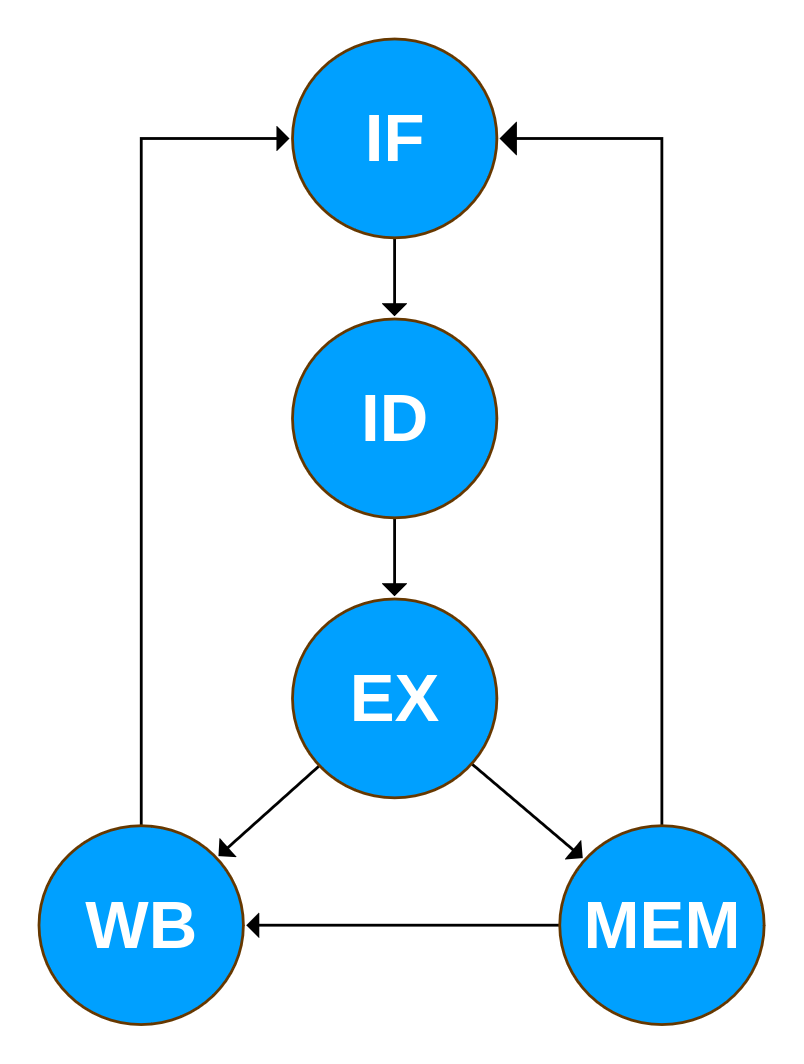
\includegraphics[width=0.6\textwidth]{media/exercise5_fsm.png}
    \caption{Σχηματικό διάγραμμα $FSM$}
\end{figure}
Κυματομορφές προσομοίωσης:
% \begin{figure}[H]
%     \centering
%     \includegraphics[width=1\textwidth]{media/exercise5_waveforms.png}
% \end{figure}

\section*{Σχόλια}
Τα εργαλεία που μας δίνονται για την ανάπτυξη υλισμικού είναι πολύ περιοριστικά σε 
σχέση με τα εργαλεία της ανάπτυξης λογισμικού που έχουμε συνηθίσει. Το $open source$ 
κίνημα δεν έχει αγγίξει τον συγκεκριμένο τομέα και αυτό έχει άμεσες συνέπειες στην 
ευχρηστία των εργαλείων. Εκτός από το $EDA Playground$ τα άλλα δύο μεγάλα σε όνομα 
εργαλεία $Quartus$ και $Ikarus$ έχουν το καθένα τους δικούς του περιορισμούς. Το 
$Quartus$ είχε μια εξαιρετικά δύσκολη διαδικασία εγκατάστασης και ενεργοποίησης, όπου 
απαιτούνταν από τον μέχρι και το $MAC$ της κάρτας δικτύου. Από την άλλη το $Ikarus$
δεν υποστηρίζει $Linux$ υπολογιστές και δεν μπόρεσα να το δοκιμάσω. Το $EDA Playground$
είναι ένα $online$ εργαλείο το οποίο ήταν εξαιρετικά βολικό στα πλαίσια της εργασίας αλλά
για μεγάλα $project$ δεν θα ήταν κατάλληλο. Κύρια μειονεκτήματα του ήταν η συνεχής,  
γρήγορη αποσύνδεση και αδυναμία επανασύνδεσης έπειτα από αδράνεια του χρήστη και η
$online$ υπόσταση του, καθιστώντας το ανίκανο να ανταπεξέλθει σε καταστάσεις που δεν 
υπάρχει σύνδεση στο διαδίκτυο. Αυτή ήταν η κύρια δυσκολία στην συγκεκριμένη εργασία. 
Αξίζει να σημειωθεί ότι η βιβλιογραφία που επισυναπτόταν με την εκφώνηση της εργασίας 
κάλυπτε πλήρως τις ανάγκες της εργασίας και ήταν εξαιρετικά χρήσιμη.
\end{document}